% !TEX root = ../../../report.tex

\FloatBarrier
\subsection{Processor Core}\label{subsec:fpga-processor-core}

This subsection describes the design considerations and the implementation of the
 processor cores in \textit{ChaosM}.

\subsubsection{Design Considerations}

The processor core in \textit{ChaosM} is designed to be able to perform audio processing in real-time, as well as being as power efficient as possible.
Since an FPGA's power usage is close to constant, the best way to save power is to reduce the time the whole board is active.
The best way for the core to contribute to this is, to execute the programs as fast as possible.
Thus, the processor core has been designed with the two following principles in mind:

\begin{itemize}
	\item As high throughput as possible.
	\item Support the instructions needed to perform the audio processing.
\end{itemize}
The resulting core design is shown in figure \ref{fig:core_schematic} below:

\begin{figure}[ht]
	\centering
	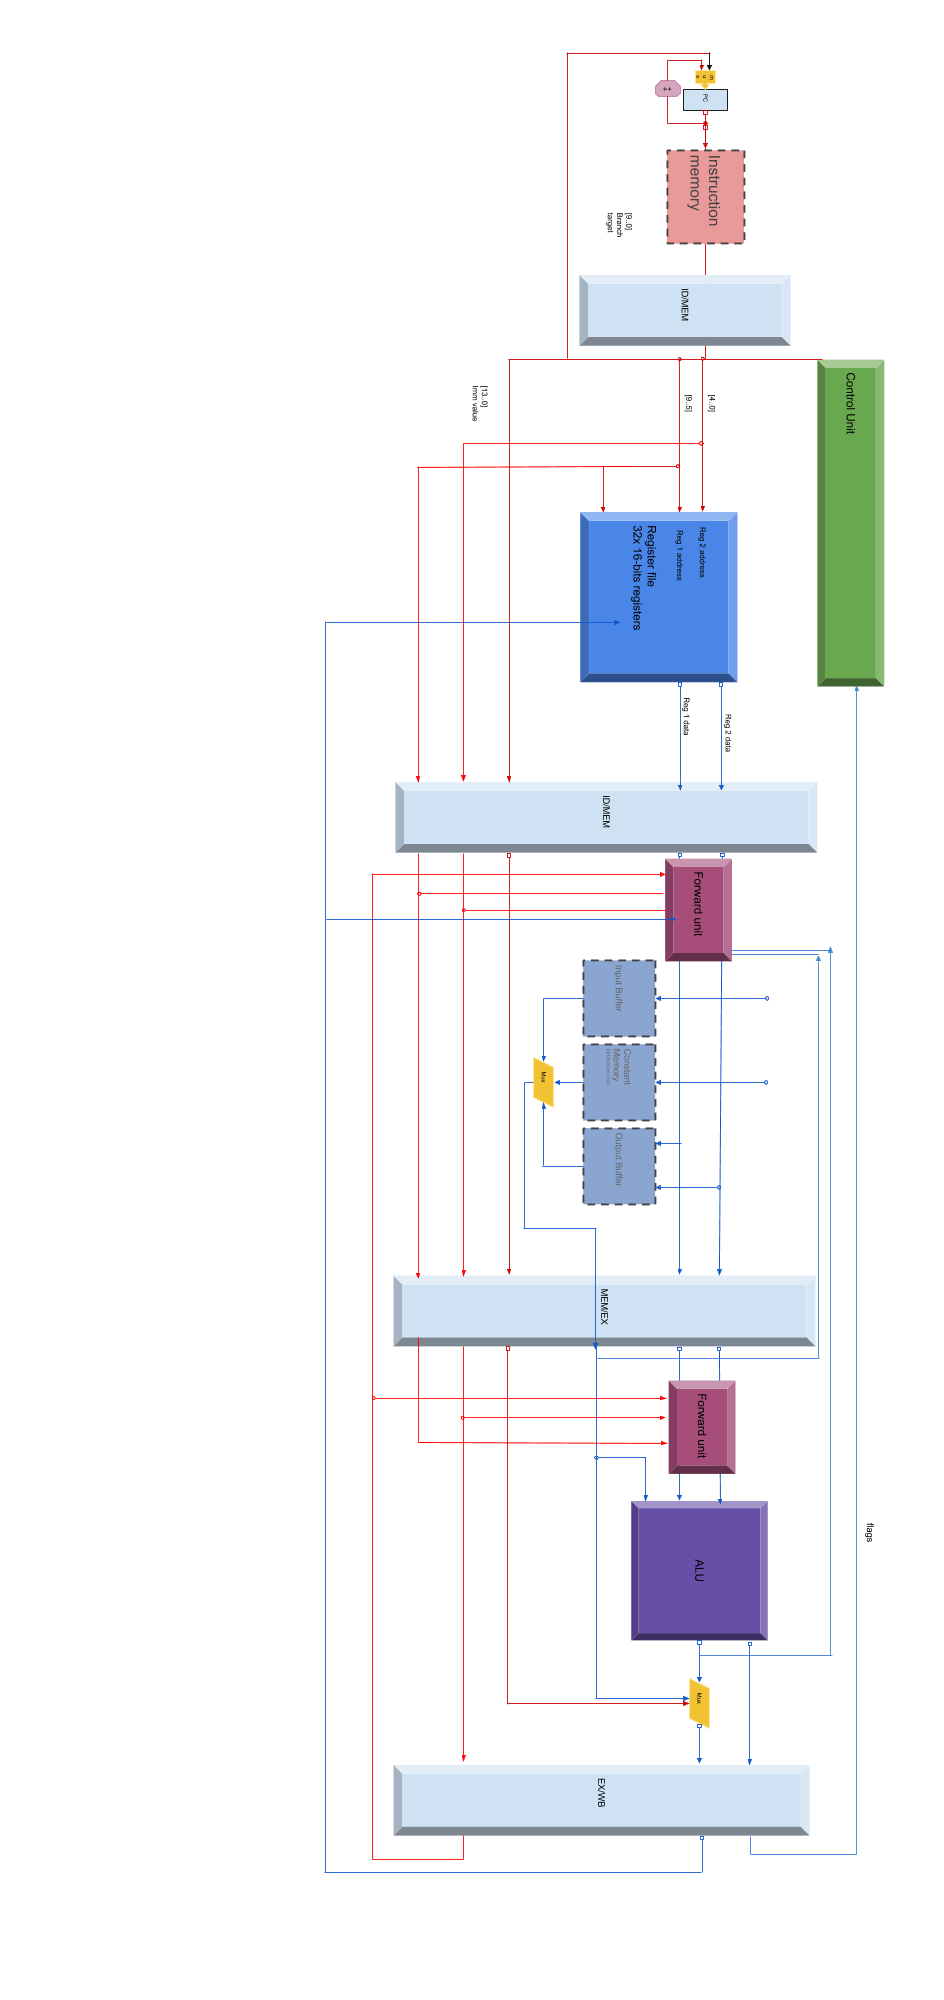
\includegraphics[width=0.8\linewidth]{figures/fpga/core_schematic}
	\caption{A simplified schematic of the processor core design.}
	\label{fig:core_schematic}
\end{figure}

\subsubsection{Implementation}

In order for the core to be as efficient as possible, a pipelined processor
design was implemented. The pipelined core design consists of the following
stages:

\begin{enumerate}
	\item Instruction Fetch \label{stage:if}
	\item Instruction Decode \label{stage:id}
	\item Memory \label{stage:mem}
	\item Execute \label{stage:ex}
	\item Write back \label{stage:wb}
\end{enumerate}

A change from the classic pipelined processor designs is that the memory stage comes before the execution stage.
This is because the load and store instructions does not need the ALU to calculate the memory address.
Thus the processor is able to prevent \textit{all} data dependecies by forwarding data from the different stages.

For simplicity, the core does not have a hazard control unit implemented for branching.
Instead it relies on the programmer to add two no-operations after a branch.

\FloatBarrier
\subsection{ALU}\label{subsection:fpga-alu}
\todo[inline]{ALU design and reasons why. -First revision finished?}

When the group sat down and started considering the ALU of our pipelined
processor cores, it was decided that we wanted to go for the ``Less is more''
design philosophy. This due to the fact that more often than not, the circuits
comprising the ALU logic tend to be the more resource-intensive and complicated
ones in a processor.

With that in mind, a following prioritization list of supported hardware
operations was made:\todo{This needs to be fleshed out when we've finished the
ALU.}
\begin{enumerate}
	\item Logic to allow for sufficiently fast Fourier-transforms (so that the
transform could be performed on each discrete sample within a single clockcycle
of the sequential processing core pipeline).
	\begin{enumerate}
		\item The Fourier-transform we settled on could be performed with only
addition, substraction, and shifting. Therefore hardware support for these
operations also had to be implemented.
	\end{enumerate}
	\item Multiplication for the sound-effect manipulations on the transformed
samples located in the frequency domain.
\end{enumerate}
\emph{For any reader potentially wondering, why division was left out, this is
explained in section \ref{subsubsection:fpga-alu-div}.}

\FloatBarrier
\subsubsection{Fourier-transforms}\label{subsubsection:fpga-alu-ft}
\todo[inline]{Need a way to refer to this subsubsection. I tried refering to it
in the design.tex file. The resulting reference refers to the ALU subsection as
a whole, and not the FT subsection.}

When it became necessary to start looking into how one implements a
Fourier-transform on a FPGA processor (as previously mentioned in section
\ref{section:fpga-design}), a lot of effort was spent on attemting to first find
examples of how others have implemented FT's (Fourier-transforms) on embedded
real-time devices before.

It did not take long before it became evident that there were two types of FT's
standing out from the rest of when considering FT's for the purpose of real-time
sound processing. Namely the Integer- and Sliding-Discrete- Fourier-Transforms.
The Integer-FT was ideal when considering that we would not have to implement
support for floating-point operations.

However, the Integer-FT needed the whole music file when transforming. It could
not transform discrete samples one at the time, which we would need if we had a
live source as input (say a portable music device connected to the PCB's
minijack). Also, we were unable to find any pseudo-code describing how such a
transform would function. The few examples we found described only the
mathematical functions, which left too huge a gap for us to research on our own.

Having found this out, the Sliding-Discrete-FTs potential use for our purposes
rose substantially. Not only would it allow us to perform a real-time
Fourier-transform, but we also managed to find pseudo-code describing how such a
transform would function. The big downside to the SD-FT however was the
necessity of floating-point to accomplish the implementation.

\FloatBarrier
\subsubsection{ALU input size}\todo{Better subsubsection title?}

Due to the algorithmically heavy operations of the SD-FT being the
\emph{heaviest} algorithmic operation performed in the the processor as a whole,
looking into how we could optimize the algorithm became a focus in the VHDL
group. Using the application \todo{Need references to actual (and correct!)
application notes here!}notes to find out the potential best speeds (read:
frequencies) of the FPGA, we then started calculating how fast the SD-FT would
have to perform its transform per sample.

It quickly became apparent that a ``quick and easy'' way to drastically reduce
the time complexity the algorithm would need to transform each sample, was to
reduce the sample sizes. \todo[inline]{Find some reference, or picture, or add a
paragraph explaining said algorithm.}With this in mind, we started testing how
small samples we could have, and yet have a passable level of sound quality. The
final result we ended up on was to have eight-bit datasamples. This had the
consequence of reducing the maximum sound frequency from ca. 44 kilohertz down
to \todo{This needs to be confirmed/edited.}11.

\FloatBarrier
\subsubsection{Leaving out division}\label{subsubsection:fpga-alu-div}

The decision to not implement hardware support for division was done for several
reasons. Firstly, hardware support for division is costly. Secondly, seeing as
we had already decided on having to implement floating-point for the SD-FT, we
decided that the amount of logic needed for each core to support both division
and floating-point was too much. Thirdly, having floating-point support, we
just as well multiply with a number smaller than one to perform a division. For
integer division it was decided that the programmer could program the cores to
perform longdivision with addition and substraction loop (or shifting when a
division by a power of 2 was attempted).

